In this chapter I am going to present the work done throughout this
project. In Section \ref{sec:fk_constraints} I will present the
database schema that we were using in Hops-YARN and how this evolved
to a schema without any foreign key constraints yet being
consistent. Section \ref{sec:tx_aggregation} gives a detailed analysis
of the new transaction state manager of Hops and how that boosted our
performance. Section \ref{sec:gc_service} deals with the garbage
collector service written for Hops that deletes asynchronously old
data from the database. Finally, in Section \ref{sec:dto_caching} we
will explore the shortcomings of the MySQL Cluster connector for Java and
how we have managed to overcome them. As I have mentioned in Chapter
\ref{chap:methods}, each feature completion was followed by a system
profiling to guide us to the next bottleneck. The order of the
performance issues identified in the system is the same as the order
of the sections that follow.

Before diving into the implementation details I would like to give a
general overview of how Hops and Hops-YARN interact with the NDB
cluster in terms of Java packages. The interaction is illustrated in
Figure \ref{fig:impl_hops_ndb}. Hops distribution is statically linked
with the Data Access Layer (DAL) package \texttt{hops-metadata-dal}
which provides an API used by both Hops-HDFS and Hops-YARN to interact
with the persistent storage. Currently we have implemented a client
library for the MySQL Cluster NDB in the package
\texttt{hops-metadata-dal-impl-ndb} which also links to the DAL
package. Our choice in favour is the NDB cluster but users are free to
implement their own client library for any other storage solution as
long as the back-end has support for transactions, read/write locks and
at least read-committed isolation. Both Hops and the DAL API are
released under an Apache 2.0 license and the DAL implementation is
licensed under GPLv2.

\begin{figure}
\centering
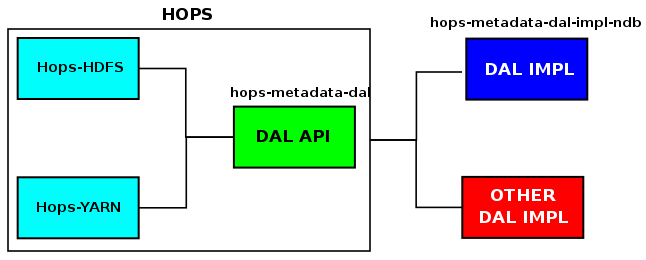
\includegraphics[scale=0.5]{resources/images/Implementation/hops_ndb_interaction.png}
\label{fig:impl_hops_ndb}
\caption{Hops - MySQL Cluster interaction}
\end{figure}
